\documentclass[12pt,spanish]{article}
\usepackage[utf8]{inputenc}
\usepackage{babel}
\usepackage{listings}
\usepackage{mathpazo}
\usepackage{enumitem}
\usepackage{courier}
\usepackage{textcomp}
\usepackage[dvipsnames]{xcolor}
\usepackage{parskip}
\usepackage{fullpage}
\usepackage{tikz}
\usetikzlibrary{arrows}

\newcommand{\onelinerule}{\rule[2.3ex]{0pt}{0pt}}
\newcommand{\twolinerule}{\rule[6.2ex]{0pt}{0pt}}
\newcommand{\respuesta}{\framebox[\textwidth]{\twolinerule}}
\newcommand{\nombre}{%
  \begin{tikzpicture}[xscale=.4,yscale=.7]
    \draw (0, 0) rectangle (22, 1);
  \end{tikzpicture}%
}
%\newcommand{\rol}   {\framebox[0.3\textwidth]{\onelinerule}}
\newcommand{\rol}{%
  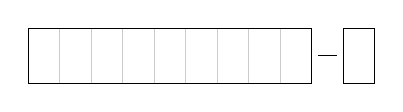
\begin{tikzpicture}[xscale=.4,yscale=.7]
    \draw[gray!40] ( 0, 0) grid      ( 9, 1);
    \draw          ( 0, 0) rectangle ( 9, 1);
    \draw          (10, 0) rectangle (11, 1);
    \draw (9 + .2, .5) -- (10 - .2, .5);
  \end{tikzpicture}%
}
\newcommand{\li}{\lstinline}
\newcommand{\pond}[1]{[{\small\textbf{#1\%}}]}

\lstdefinelanguage{py}{%
  classoffset=0,%
    morekeywords={%
      False,class,finally,is,return,None,continue,for,lambda,try,%
      True,def,from,nonlocal,while,and,del,global,not,with,print,%
      as,elif,if,or,yield,assert,else,import,pass,break,except,in,raise},%
    keywordstyle=\color{black!80}\bfseries,%
  classoffset=1,
    morekeywords={int,float,str,abs,len,raw_input,exit,range,min,max,%
      set,dict,tuple,list,bool,complex,round,sum,all,any,zip,map,filter,%
      sorted,reversed,dir,file,frozenset,open,%
      array,zeros,ones,arange,linspace,eye,diag,dot},
    keywordstyle=\color{black!50}\bfseries,%
  classoffset=0,%
  sensitive=true,%
  morecomment=[l]\#,%
  morestring=[b]',%
  morestring=[b]",%
  stringstyle=\em,%
}

\lstdefinelanguage{testcase}{%
  moredelim=[is][\bfseries]{`}{`},%
  backgroundcolor=\color{gray!20},%
}

\lstdefinelanguage{file}{%
  frame=single,%
  backgroundcolor=\color{white},%
}

\lstset{language=py}
\lstset{basicstyle=\ttfamily}
\lstset{columns=fixed}
\lstset{upquote=true}
\lstset{showstringspaces=false}
\lstset{rangeprefix=\#\ }
\lstset{includerangemarker=false}

\newlist{certamen}{enumerate}{1}
\setlist[certamen]{%
  label=\arabic*.,
  font=\LARGE\bfseries,%
  labelindent=-.5in,%
  leftmargin=0pt,%
  labelsep=1em%
}



%\lstset{language=testcase,frame=single}
\lstset{language=py}

\begin{document}
  \thispagestyle{empty}
  \pagestyle{empty}
  \section*{Lunes 1 de octubre}

%  \emph{%
%    Para la actividad de hoy
%    es prerrequisito haber leído los siguientes capítulos de la materia:
%    Funciones, Módulos, Listas y Tuplas.
%  }

  \begin{minipage}[T]{0.7\textwidth}
    \parskip=2ex
    Un punto \((x, y)\) del plano
    puede ser representado en un programa
    como una tupla de dos valores \li!(x, y)!.
    Un polígono puede ser representado como la lista de sus vértices.

    Por ejemplo,
    el polígono de la derecha
    quedaría representado de la siguiente manera:
    \begin{lstlisting}
p = [(40, 40), (50, 0), (20, 10),
     (10, -10), (-10, 0), (0, 30)]
    \end{lstlisting}
  \end{minipage}
  \hfill
  \begin{minipage}[T]{0.25\textwidth}
    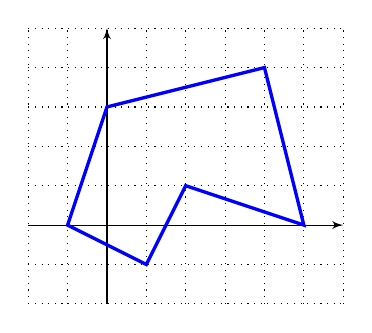
\begin{tikzpicture}[scale=0.5]
      \draw[dotted] (-2, -2) grid (6, 5);
      \draw[-latex'] (-2, 0) -- (6, 0);
      \draw[-latex'] (0, -2) -- (0, 5);
      \draw[very thick, Blue]
            ( 4, 4) --
            ( 5, 0) --
            ( 2, 1) --
            ( 1, -1) --
            (-1, 0) --
            ( 0, 3) --
            cycle;
    \end{tikzpicture}
  \end{minipage}

  En la actividad de hoy,
  su equipo debe desarrollar un módulo llamado \texttt{poligonos.py},
  que contenga las siguientes funciones para manipular polígonos.

  \begin{enumerate}[leftmargin=0pt]

    \item La función \li!numero_de_lados(p)!
      retorna la cantidad de lados que tiene el polígono \li!p!:
      \lstinputlisting[linerange=LADOS-FIN\ LADOS]{casos.txt}

    \item La función \li!distancia(a, b)!
      retorna la distancia entre los puntos \li!a! y \li!b! del plano.
      \lstinputlisting[linerange=DISTANCIA-FIN\ DISTANCIA]{casos.txt}

    \item La función \li!calcular_perimetro(poligono)!
      retorna el perímetro del \li!poligono!.
      \lstinputlisting[linerange=PERIMETRO-FIN\ PERIMETRO]{casos.txt}

    \item La función \li!dibujar(poligono)!
      dibuja el \li!poligono! usando la tortuga.
      (Las funciones \li!up()!, \li!down()! y \li!goto(x, y)!
      del módulo \verb!turtle! le serán útiles).

      \includegraphics[width=\textwidth]{p1}

    \item La función \li!trasladar(poligono, dx, dy)!
      traslada el \li!poligono! completo,
      moviéndolo \li!dx! unidades horizontalmente
      y \li!dy! unidades verticalmente.

    \item La función \li!escalar(poligono, factor)!
      escala el tamaño del \li!poligono!
      en el \li!factor! indicado.

      \includegraphics[width=\textwidth]{p2}

    \item
      \emph{(Opcional).}
      La función \li!crear_poligono_regular(n, a)!
      retorna un polígono regular de \li!n! lados
      de largo \li!a!.

    \item
      \emph{(Opcional).}
      La función \li!encerrar(poligono)!
      dibuja un rectángulo que encierra al \li!poligono!.

      \includegraphics[width=\textwidth]{p3}

  \end{enumerate}




\end{document}

